\documentclass[10pt, preprint, nocopyrightspace]{sigplanconf}

% The following \documentclass options may be useful:

% preprint      Remove this option only once the paper is in final form.
% 10pt          To set in 10-point type instead of 9-point.
% 11pt          To set in 11-point type instead of 9-point.
% authoryear    To obtain author/year citation style instead of numeric.

\usepackage{amsmath}
\usepackage{amssymb}
\usepackage{listings}
\usepackage{hyperref}
\usepackage{subcaption}
\usepackage{todo}

\special{papersize=8.5in,11in}
\setlength{\pdfpageheight}{\paperheight}
\setlength{\pdfpagewidth}{\paperwidth}

\lstset{captionpos=b, float, language=python}

\usepackage{tikz}
\usetikzlibrary{positioning}
\usetikzlibrary{shadows}
\usetikzlibrary{arrows}
\usetikzlibrary{shapes}
\usetikzlibrary{calc}

\providecommand{\boostsimd}{\textsc{Boost.SIMD}}
\providecommand{\cpp}[1][~]{\textsc{C++}#1}
\providecommand{\ie}[1][~]{\textit{i.e.}#1}
\providecommand{\eg}[1][~]{\textit{e.g.#1}}


\begin{document}


\title{Efficient Compilation of High Level Python Numerical Programs with Pythran}

\authorinfo{Serge Guelton}
{T{\'e}l{\'e}com Bretagne}
{serge.guelton@telecom-bretagne.eu}
\authorinfo{Pierrick Brunet}
{INRIA/MOAIS}
{pierrick.brunet@inria.fr}
\authorinfo{Mehdi Amini}
{Apple}
{mehdi.amini@apple.com}

\maketitle

%\begin{abstract}
%
%    For decades, FORTRAN and C(++) have dominated the landscape of High
%    Performance Computing languages, leaving interpreted language like Matlab,
%    R, Python or more recently Julia for experimentation and prototyping.
%
%    As more scientists use these scripting languages, there is an on-going
%    research effort to compile them into efficient native code. However these
%    languages favor a high-level coding style, so the computation kernels are
%    different from those used in traditional C or Fortran programs:
%    explicit raw loops are replaced by high-level constructs and calls to the
%    relevant toolbox/module/library/package. As a consequence, traditional
%    algorithms to perform loop optimization techniques like fusion, tiling and
%    related vectorization or parallelization techniques are not directly
%    applicable.
%
%    This papers focuses on the case of the Python language and especially the
%    Numpy package that provides core array data structure and basic linear
%    algebra routines. It first conducts a case study based on Numpy use
%    cases from the StackOverflow questions and answers website, then studies
%    existing compilers for numerical Python. Optimization opportunities,
%    including parallelization and vectorization, and their implementation in
%    the Pythran compiler are presented and illustrated through several
%    benchmarks, showing very interesting speedups over the standard Python
%    interpreter. Speedup greater than a factor of 10 are achieved despite the
%    fact that the considered benchmarks mostly call Numpy routines that run C code.
%
%\end{abstract}
%
%
%\keywords
%Static Compilation, Parallelization, Python, C++, SIMD, Runtime

%%
%%
\section*{Abstract}
% On aura pas le temps pour le papier je pense mais faire une comparaison avec
% du C pure pour voir ce que les compilo de C arrive a faire.

The Python language~\cite{rossum97} has a rich ecosystem that now provides a
full toolkit to carry out scientific experiments, from core scientific routines
with the Numpy package\cite{oliphant2007,numpyarray2011}, to scientific
packages with Scipy, plotting facilities with the
Matplotlib package, enhanced terminal and notebooks with IPython. As a
consequence, there has been a move from historical languages like Fortran to
Python, as showcased by the success of the Scipy conference.

As Python based scientific tools get widely used, the question of High
performance Computing naturally arises, and it is the focus of many recent
research. Indeed, although there is a great gain in productivity when using
these tools, there is also a performance gap that needs to be filled.

This extended abstract focuses on compilation techniques that are relevant for the
optimization of high-level numerical kernels written in Python using the Numpy
package, illustrated on a simple kernel.

%% Its introduces the implementation of these techniques in the Pythran
%% compiler and provides a benchmark test suite for performance measures along
%% several Python compilers.
%% Section~\ref{sec:stackoverflow} presents a case study based on user
%% input gathered from the StackOverflow questions and answers website.
%% Section~\ref{sec:optimize} focuses on a simple yet representative kernel and
%% showcases the optimization opportunities typically found in Numpy-based
%% kernels. Existing compilation approaches to optimize such kernels are discussed
%% in Section~\ref{sec:compilers}. Section~\ref{sec:pythran} emphasises on
%% compiler-runtime cooperation to solve the performance issues.
%% Finally, experimentations showcasing important performance gains are detailed in
%% Section~\ref{sec:xp}.


%%% %%
%%% %%
%%% \section{A Crowd-Sourced Numpy Benchmark}
%%% \label{sec:stackoverflow}
%%% 
%%% One of the first steps required when designing an optimizing compiler is to
%%% gather enough test cases, or benchmarks, in order to drive the optimization
%%% process toward realistic examples. To achieve this goal, we have gathered a few
%%% examples from existing compilers' test suites, but these may have been modified to
%%% overcome some compiler limitations. A less biased source of benchmarks should
%%% be independent from the compiler community and showed focus on matching user needs.
%%% To achieve that goal, we collected synthetic scientific kernels from the
%%% StackOverflow website.
%%% 
%%% StackOverflow\footnote{\url{http://stackoverflow.com/}} is a question and
%%% answer site for programmers. Any registered user can submit questions and other
%%% users may answer. A voting system is then used to sort the answers. Said
%%% otherwise, the website provides a database of questions and answers on
%%% programming topics, including Python.
%%% 
%%% A query using the terms \emph{numpy} and \emph{slow} yields a lot of results, many
%%% of which expose the pattern ``Q: my code is slow'' followed by an upvoted answer
%%% ``A: rewrite it that way'', where the original code performs explicit looping
%%% over an array, and the rewritten code uses the relevant combination of Numpy
%%% function.
%%% 
%%% For instance, question \href{http://stackoverflow.com/questions/7741878}{7741878}
%%% proposes to use an explicit loop to iteratively compute the $L^2$ norm of each
%%% row of a matrix, as illustrated in Listing~\ref{lst:l2norm-loopy}, and one of
%%% the proposed answer is to use the more compact version presented in
%%% Listing~\ref{lst:l2norm}. This answer no longer uses any explicit loop and
%%% roughly achieves a $\times 4$ speedup over the loop version.
%%% 
%%% \begin{lstlisting}[language=python,caption={Per row version of $L^2$ norm with loop in Numpy.}, label={lst:l2norm-loopy}]
%%% def l2norm_slow(x):
%%%     r = np.empty(x.shape[0])
%%%     for i in xrange(x.shape[0]):
%%%         r[i] = np.sum(np.abs(x[i])**2)
%%%     return r
%%% \end{lstlisting}
%%% 
%%% \begin{lstlisting}[language=python,caption={Per row version of $L^2$ norm without loop in Numpy.}, label={lst:l2norm}]
%%% import numpy as np
%%% def l2norm_fast(x):
%%%     return np.sum(np.abs(x)**2, axis=1)
%%% \end{lstlisting}
%%% 
%%% Newcomers to Python with a prior C or Fortran experience are likely to make
%%% use of raw loops similar to Listing~\ref{lst:l2norm-loopy}, but as their
%%% knowledge of the Numpy API and of good programming practices grows, they get to 
%%% write code similar to Listing~\ref{lst:l2norm}. 
%%% The fact that Numpy high-level constructs runs faster is also a strong 
%%% motivation. As a direct consequence, a compiler should focus on optimizing
%%% high-level constructs rather than raw
%%% loops. Both to encourage good practice with respect to Numpy code, and because
%%% this is the kind of code Numpy users ultimately write.
%%% 
%%% A selection of benchmarks collected during this process, selected for their
%%% conciseness and representativity of high-level calls, are publicly available on
%%% \url{https://github.com/serge-sans-paille/numpy-benchmarks}, with a set of
%%% benchmarking routines specialized for major Python/Numpy compilers. This
%%% benchmark is used in \S~\ref{sec:xp} to evaluate the validity of the approach
%%% described in this paper.


%%
%%
\section{Optimizations Opportunities in a Typical Numpy Kernel}
\label{sec:optimize}

This section briefly presents the core concepts of the Numpy package, then goes
through all the optimization opportunities in a small kernel as a showcase of
the optimization opportunities.

\subsection{Numpy}

The reference implementation of Numpy is a native Module, written mostly in C.
It uses the BLAS API whenever possible and provides a relatively efficient array
abstraction in the form of the \texttt{ndarray} data structure.

%% This data
%% structures makes it possible to use various styles of slicing and broadcasting,
%% as illustrated in Listing~\ref{lst:pairwise}.

It also enforces a high-level programming style but it's very inefficient when
explicit subscripts are used. 

%% For instance, raw loops are used in
%% Listing~\ref{lst:pairwise-raw}. It avoids the creation of temporary arrays but
%% runs almost 100 times slower due to the Python interpreter overhead and the C
%% to Python conversion involved in every subscript.
%% 
%% \begin{lstlisting}[language=python, caption={\textit{pairwise} function that
%%   exhibits array broadcasting.}, label={lst:pairwise}, breaklines=true]]
%% def pairwise_numpy(X):
%%     return np.sqrt(((X[:, None, :] - X) ** 2).sum(-1))
%% \end{lstlisting}
%% 
%% 
%% \begin{lstlisting}[language=python, caption={\textit{pairwise} function
%%   using raw loops.}, label={lst:pairwise-raw}]
%% def pairwise_python(X):
%%     M = X.shape[0]
%%     N = X.shape[1]
%%     D = np.empty((M, M), dtype=np.float)
%%     for i in range(M):
%%         for j in range(M):
%%             d = 0.0
%%             for k in range(N):
%%                 tmp = X[i, k] - X[j, k]
%%                 d += tmp * tmp
%%             D[i, j] = np.sqrt(d)
%%     return D
%% \end{lstlisting}

\subsection{The Rosenbrock Function}

We use the kernel illustrated in Listing~\ref{lst:rosen} and adapted from the
Scipy source code of \texttt{scipy.optimize.rosen} as a leading example. It
uses Numpy's \texttt{sum} function, Python's square notation and Numpy's array
slicing. It is a good example of high-level Python kernel, although using the
original function directly would naturally make sense.

Note that due to dynamic typing, this function can take arrays of different
shapes and types as input.

\begin{lstlisting}[language=python, caption={High-level implementation of the Rosenbrock function in Numpy.}, label={lst:rosen}]
def rosen(x):
    t0 = 100 * (x[1:] - x[:-1] ** 2) ** 2
    t1 = (1 - x[:-1]) ** 2
    return numpy.sum(t0 + t1)
\end{lstlisting}


\subsection{Temporaries Elimination}
\label{sec:temporaries-elimination}

In Numpy, any point-to-point array operation allocates a new array that holds
the computation result. This behavior is consistent with many Python standard
module, but it is a very inefficient design choice, as it keeps on polluting
the cache with potentially large fresh storage and adds extra
allocation/deallocation operations, that have a very bad caching effect. In the
\textit{rosen} function from Listing~\ref{lst:rosen}, 7 temporary arrays are
allocated (slicing does not create a temporary array but a view) to hold
intermediate steps. Had the expression been evaluated lazily, no temporary
would have been needed.

\subsection{Operator Fusion}
\label{sec:operator-fusion}

As Numpy is a native library mostly written in C, each operator computation is
performed by a function implemented as a loop performing a single operation,
and the operator chaining is done at the interpreter level. This is a typical
problem in library design: if only a small set of functions is provided, it
prevents the optimization of merging multiple operators into a single specialized
operator. On the contrary, providing many operator combinations as part of the library yields
better performance to the price of API bloat. Listing~\ref{lst:rosen}
illustrates the use of a small set of functions: a loop is generated for
each temporary computation, plus an extra loop for the \texttt{numpy.sum}
reduction, whereas a single loop would have been necessary with operator fusion.

\subsection{Loop Vectorization and Parallelization}

Without operator fusion, there would be very little benefit to generate SIMD
instructions for the respective array operations used by each operator, as the
memory loads and stores would have dominated the execution time. This is even more important as
Numpy typically operates on double precision floats, which means only two (SSE)
to four (AVX) scalars per vector registers.

Parallelization would also suffer from the lack of operator fusion: a
synchronization fence is needed between each temporary computation.  Hence the
loop computation intensity would be very low compared to the memory pressure
implied by two array reads and one array write for a single binary operator.

On the opposite, if all computations were merged into a single loop using
temporaries elimination and operator fusion, parallelization would be more
effective as barriers between binary operations are no longer needed and loads
and stores are counterbalanced by several operations.

%%
%%
\section{Optimization with the Pythran Compiler}

\subsection{Pythran}

The optimizations presented in the previous section have been implemented in the Pythran
compiler~\cite{pythran2013}, a translator from a subset of Python to
C++11~\cite{isocxx11}. The input Optimization a Python module written in
the subset accepted by the compiler. Pythran translates it in its internal representation, a
simplified Python AST. It performs various optimizations then outputs either
Python code, in a source-to-source fashion, or C++ templated code calling the pythonic library that typically implements the \texttt{ndarray}
interface. User annotations can be used to instantiate this code for the proper
types and generate a native library. This library relies on Boost.Python
library to match Python's C API.

The Pythran compiler is an open source project publicly released under the BSD
license\footnote{\url{http://pythonhosted.org/pythran/}}.

Compared to existing alternatives, Pythran keeps the static compilation
approach used by Cython, when JIT compilation is mainly used to statically type
kernels before code generation in Numba and Parakeet. Unlike Cython, it
maintains full Python backward compatibility.  Following the Parakeet approach,
it focuses on high-level constructs, while still generating efficient code for
explicit loop and subscripts.



%%
%%
\subsection{Experiments} \label{sec:xp}

The experiments are run on an Intel(R) Xeon(R) CPU E5-2650 0 @ 2.00GHz for a
total of 8 cores (multithreading is not used). Each node has access to 64\,KB
of L1 cache, 256\,KB of L2 cache. Both L1 and L2 caches are private, while L3
cache is shared between the 8 cores. This configuration provides a total of
64\,GB of main memory. It supports up to AVX. The backend compiler is GCC 4.9
(20140528) with libgomp.

To compare the different optimization effects, we evaluated different
optimization combination for Listing~\ref{lst:rosen}. The input is a raw array
of 1,000,000 single precision floating point elements.
Figure~\ref{fig:rosenintel8} illustrates the results. We can notice the
importance of forward substitution on this benchmark as we avoid one extra
loop, two temporary array assignments and some load/store for SIMD
instructions. Vectorization is also extreemly profitable.

\begin{figure}[t]
\centering
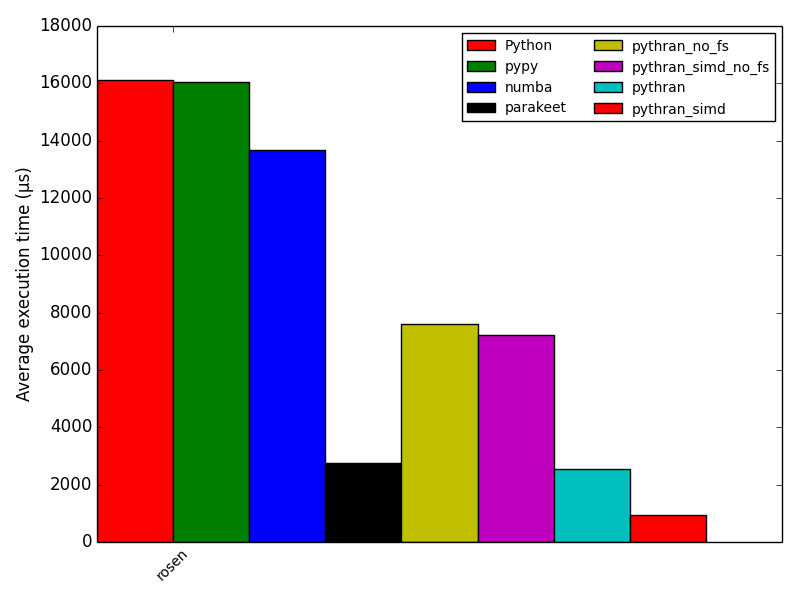
\includegraphics[width=.5\textwidth]{rosen_intel8.png}
\caption{Execution time of the rosen kernel on Intel Xeon.}
\label{fig:rosenintel8}
\end{figure}

%%
%%
\section*{Conclusion}

This extended abstract presents a short study of the optimization of Python/Numpy high level
kernels in the context of high performance computing. It uses a real-worl synthetic kernel as leading example and focuses on the efficient
implementation and optimization of array expressions within the ahead-of-time
Pythran compiler, showing that a compilation step at Python level before
generation of lower-level code makes it possible to generate vectorized,
parallel C++ code. A comparison with existing JIT compilers for scientific
Python validates the approach, showing significant performance improvements
over the state of the art.

\acks

The Pythran project was partially funded
by the CARP Project and the SILKAN Company.

%Several Students of Télécom Bretagne, namely Adrien Merlini, Alan Raynaud,
%Xavier Corbillon, Yuancheng Peng and Eliott Coyacc, have made significant
%contributions to the project.

% The authors are very grateful to Béatrice Creusillet for her careful proof reading.

% We recommend abbrvnat bibliography style.

\bibliographystyle{abbrvnat}
\bibliography{biblio}


\end{document}
